\documentclass[12pt,oneside]{book}

\usepackage[dvips,letterpaper,margin=0.75in,bottom=0.75in]{geometry}
\usepackage{cite}
\usepackage{slashed}
\usepackage{graphicx}
\usepackage{amsmath}
\usepackage{enumitem}
\usepackage{amsthm}
\theoremstyle{definition}

\usepackage[american,fulldiode]{circuitikz}
\tikzset{component/.style={draw,thick,circle,fill=white,minimum size =0.75cm,inner sep=0pt}}
\newtheorem{measurement}{Logbook Entry}[chapter]
\newtheorem{plot}{Jupyter Notebook}[chapter]

\begin{document}
\ctikzset{bipoles/thickness=1}
\ctikzset{bipoles/length=.6cm}

\title{Python Exercises}
\maketitle
\chapter{Probability Distributions}

%
% TODO:  Students were confused about how to handle bin position
% for plotting discrete data...  some clarification (text, figures) is needed.
%

\section{Introduction}

In this lab, you will create your own numerical simulation of a binomial
process, and compare the results of your simulation with the PDFs for
the binomial, Poisson, and Gaussian processes in the appropriate
limits.  For this lab there are only jupyter notebook entries. 


This lab includes a number of code snippets to illustrate the ideas
that are being discussed.  However, the entire source listing is not
available to you, as this would amount to giving away the answer, and
we all learn best by doing things ourselves!  The examples should
help you understand what you should do, but you will have to write
your own code.  {\bf Do not expect the code snippets as written to
  simply work for your code without any modification... they are not
  intended to!}

\section{Simulating the Binomial Process}

Your first task is to create a Monte Carlo simulation for a binomial
process.  The Monte Carlo method, named after the casino in Monaco, refers
to the repeated sampling of random variables to obtain numerical results.

Suppose one single experiment consists of $n_{\rm try}$ trials with a
probability $\epsilon$ of success.  The outcome of each experiment is
a single number from 0 to $n_{\rm try}$ reporting the number of the
$n_{\rm try}$ trials from that particular experiment which were
successful.  To study the distribution of outcomes, you will repeat the
experiment $n_{\rm exp}$ times.

There are library functions that will simulate this process for you,
but for this lab you will create your own simulation.  While
developing your code, start with a small test. For instance $n_{\rm
  try} = 3$ and $n_{\rm exp}=5$, as shown in the example below.
Implement your Monte Carlo simulation in the following manner:
\begin{itemize}
\item Create a 2-D array of shape $n_{\rm exp}$ by $n_{\rm try}$
  filled with random values chosen uniformly from 0 to 1.0:\\
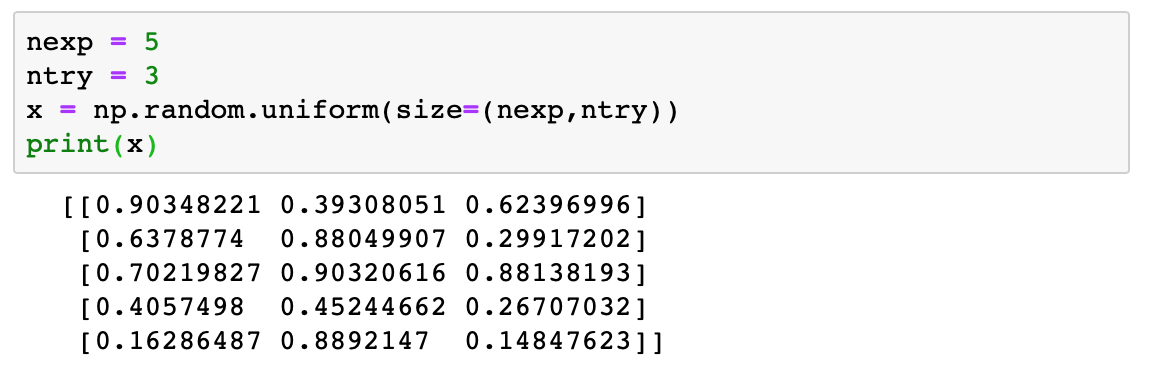
\includegraphics[width=0.85\textwidth]{figs/labs/distributions/makearray.png} \\
This array associates a random value with each trial from each
experiment.  
\item Consider a trial successful if the randomly chosen value is less
  than $\epsilon$.  In this example, taking $\epsilon = 0.5$ and
  assuming 1 indicates success and 0 a failure, we obtain:
\begin{samepage}
\begin{verbatim}
[[0 1 0]
 [0 0 1]
 [0 0 0]
 [1 1 1]
 [1 0 1]]
\end{verbatim}
\end{samepage}
In the first simulated experiment, only the second trial was
successful.  In the second experiment, only the last trial successful.
And so on.

\item Next, count the number of trials that were successful in each experiment.  The result will be a 1-D array of length $n_{\rm exp}$.  Consider using the {\tt np.sum} function with the {\tt axis} parameter (If documentation is unclear to you, check the examples).    In this example, we obtain the array of outcomes $m$:
\begin{verbatim} 
[1 1 0 3 2]
\end{verbatim}
This is the outcome of our five simulated experiments.  The first
and second experiment have one out of three trials successful, the third
experiment had zero out of three trials successful, and so on.
\end{itemize}

Work through the example and make sure you see how each result follows
from the previous step.  Then implement and test your own version of
this algorithm in Scientific Python.  If you are an experienced
programmer, you should put your simulation into a function like:
\begin{verbatim}
    def throw_binomial(nexp,ntry,eps):
       x = np.random.uniform(size=(nexp,ntry))
       #...your simulation follows...    
\end{verbatim}
This will make your code much easier to manage, because you can simply call this function each time you need to run your simulation, but it is optional.  Cutting and pasting is also permissible.


When validating a numerical calculation, think hard about good test
cases.  For instance, if you only test with the value of $\epsilon =
0.5$, you won't catch a bug that mistakes success for failure.  Try a
few different test cases, with reasonably small values for $n_{\rm
  try}$ and $n_{\rm exp}$ and check your numerical simulation.
Boundaries often make a good check, for instance $\epsilon = 0$ and
$\epsilon = 1$.

Another effective validation strategy is to check known mathematical
relations using your simulation.  For instance, we know that the mean
value of a Binomial distribution is given by:
\begin{equation} \label{eqn:binom_mean}
\bar{m} = n_{\rm try} \cdot \epsilon
\end{equation}
and that the variance is given by:
\begin{equation} \label{eqn:binom_var}
\sigma^2 = n_{\rm try} \cdot \epsilon \, (1 - \epsilon)
\end{equation}
and so these predicted values, calculated from your parameters
$\epsilon$ and $n_{\rm try}$ can be compared to the mean and variance
of the outcome array $m$ from your simulation, calculated using the numpy functions {\tt np.mean} and {\tt np.var}.  A
comparison with $n_{\rm exp}=1000$, $n_{\rm try}=10$, and
$\epsilon=0.5$ should result in something like:\\
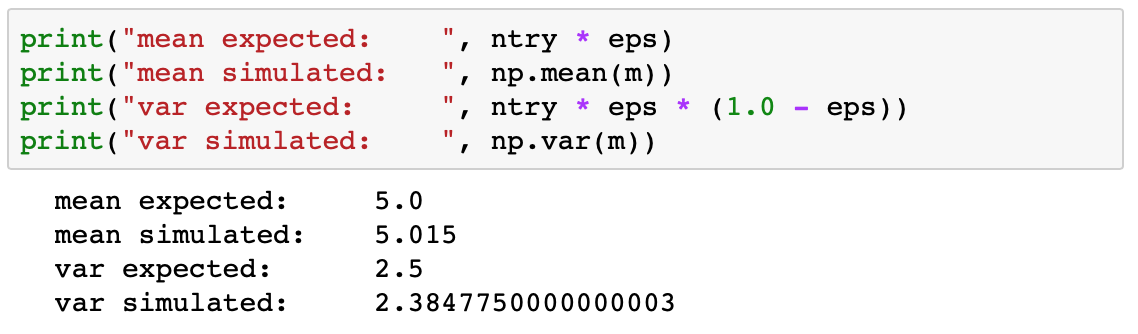
\includegraphics[width=0.8\textwidth]{figs/labs/distributions/validate.png}\\ 

\begin{print} Produce a large number of pseudo-experiments by setting $n_{\rm exp} =
1000$ and comment out any debugging print statements which will get
very long.  Pick two  well chosen test cases with different values of
$n_{\rm try}$ and $\epsilon$ and compare the expected and simulated
mean and variances. 

%Not really visual since it fluctuates and one would need to study the average behaviour for this
%Print also the values for the percent error for mean and variance
%\begin{equation}
%\mbox{percent error}= \frac{|\mbox{expected}-\mbox{simulated}|*100\%}{\mbox{expected}}
%\end{equation}

 The simulated values will fluctuate by a
fractional amount $1/\sqrt{n_{\rm exp}}$.  So for $n_{\rm exp} =
1000$, we expect the expected and simulated values to agree within
about $3\%$.  If you increase to $n_{\rm exp} = 100000$, the agreement
should improve to better than $1\%$.  Be certain to print your test
cases and the results in a clear way in your notebook. \end{print}

\section{Histogram for the Binomial Process}

We use histograms to represent the distribution of numerical data.  In
this case, our histogram simply reports the number of times each particular outcome
occurs.  Fill an output array $m$ with the simulated results of $n_{\rm exp} =
1000$ experiments each consisting of $n_{\rm try}=10$ trials with
success rate $\epsilon=0.25$.  There are eleven possible outcomes for
each of these experiments: $0,1,2,\ldots,10$.  We want to know how
often each of these outcomes occurred.

\begin{plot} Construct and plot a histogram from your simulated results in array $m$ using the 
{\tt np.histogram} function: \end{plot}
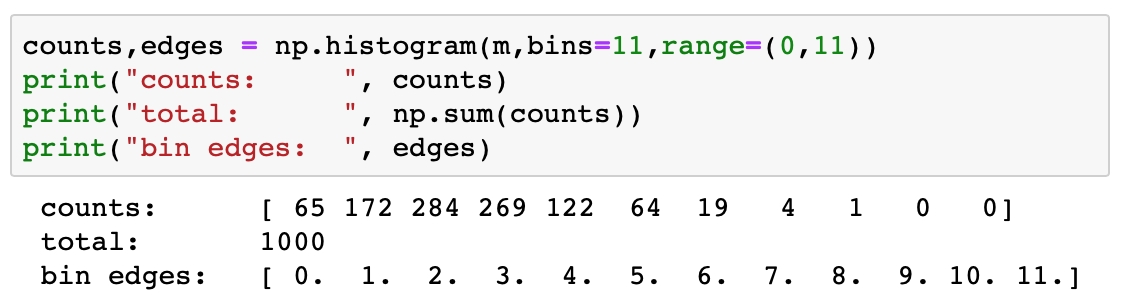
\includegraphics[width=0.8\textwidth]{figs/labs/distributions/makehist.png}\\ 
This calculates a histogram with eleven bins covering the range
from zero to eleven, and reports the number of outcomes from $m$ that
occur in each bin.  It returns two arrays, which we save as 
{\tt counts} and {\tt edges}.  We interpret the {\tt counts} array as
follows: the first entry tells us that 65 experiments had zero
successes, the second entry that 172 experiments had one success, the
third entry that 284 experiments had two successes, and so on.  The
exact values will vary each time you run the simulation, but in all
cases the sum across all bins will equal the total number of
experiments $n_{\rm exp} = 1000$.

Histograms are most often used to handle continuous data, so you
have to take a bit more care when using them to display discrete data
(integers) as we are doing here.  Consider the bin edges array {\tt
  edges} that was returned in this example:
\begin{verbatim}
   bin edges:   [ 0.  1.  2.  3.  4.  5.  6.  7.  8.  9. 10. 11.]
\end{verbatim}
which you will notice has length 12.  This is because the
array contains the {\bf edges} of eleven consecutive bins.  Technically the first bin
is the count of all outcomes in the range from zero (inclusive) to
just below one (exclusive).  The next bin is the count of all outcomes
in the range from one (inclusive) to just below two (exclusive).  In
this case, however, we are using discrete data, and so there are no entries with values like 1.73 to consider.
All the entries in the first bin are from experiments with the outcome
zero, while all the entries in the second bin are from the outcome
one.  The best way to plot this histogram, therefore, is
to associate each count with the leading bin edge, that is:\\
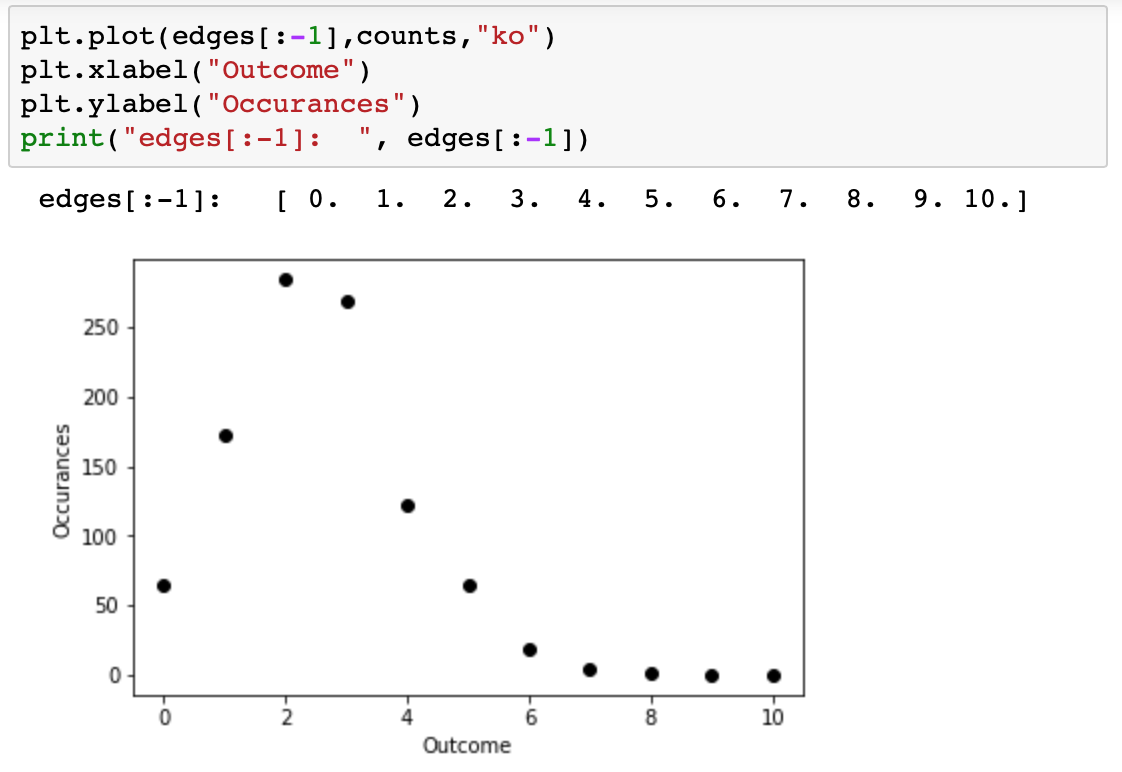
\includegraphics[width=0.8\textwidth]{figs/labs/distributions/plothist.png} \\
Notice the essential trick for plotting histogram with discrete data in integer bins is to use the slice {\tt edges[:-1]} of the bin edges data
\begin{verbatim}
   edges[:-1]:   [ 0.  1.  2.  3.  4.  5.  6.  7.  8.  9. 10.]
\end{verbatim}
as the $x$ values for plotting the occurrences of each outcome.  This
slice (all but the last entry) essentially throws out the superfluous
bin edge 11.  As we will see later, this trick only works for discrete
data in integer bins.  Notice that in resulting plot, we have the number of occurances
at each of the eleven possible outcomes correctly centered over the
numbers $0,1,2,\ldots,10.$

\section{Error Bars}

\begin{plot} Add error bars to your histogram and make a new plot.
\end{plot}
Run your simulation a few times and you will observe that the
simulated values fluctuate slightly each time you run your code.  But
how much should we expect these values to fluctuate?  If you consider
a single bin of your histogram in isolation, it contains a single
count $N$, which is itself the result of a simple counting experiment.
Counting experiments are described by the Poisson distribution.  Our
best estimate for the mean value $\lambda$ of this counting experiment
is simply our count $N$.  For the Poisson distribution the variance
$\sigma^2=\lambda$, and so we expect $\sigma = \sqrt{\lambda} =
\sqrt{N}$.  We expect each bin in our histograms to fluctuate by an
amount $\sigma$ which is the square root of the value of the bin.

To aid in interpreting histograms, it is useful to indicate the amount
we expect each bin to fluctuate by adding to the data point an ``error
bar'' with a length equal to the square root of the size of the number
of events in the
bin:\\ 
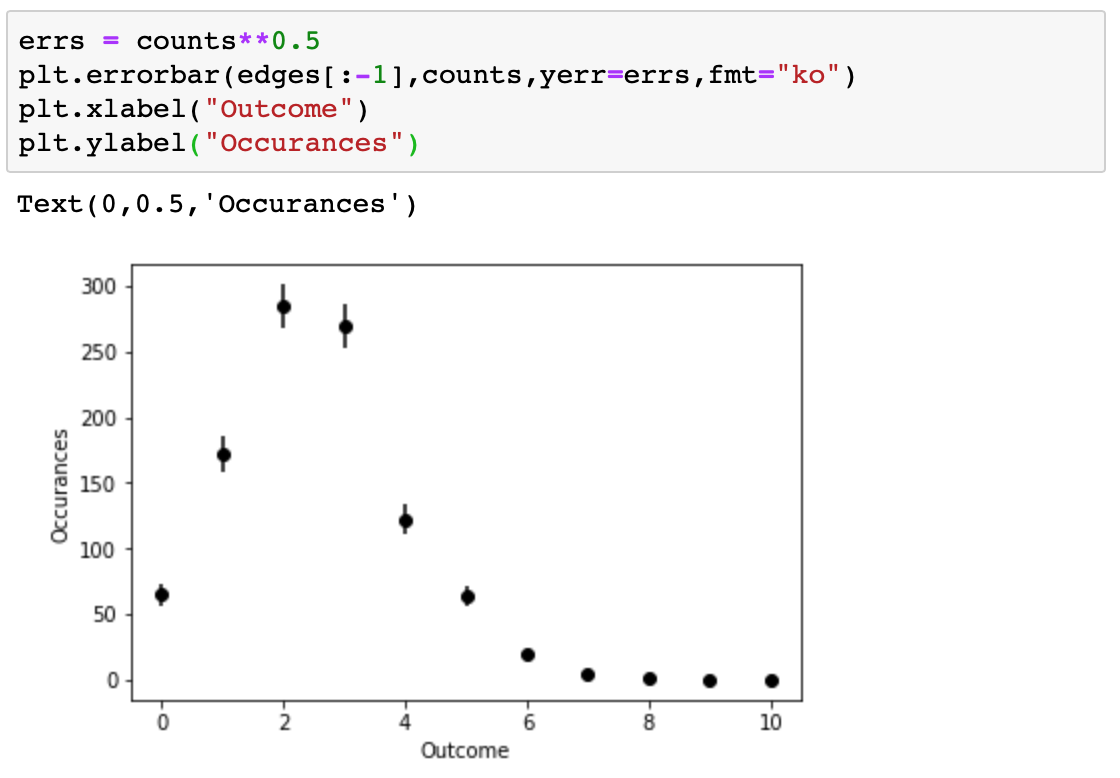
\includegraphics[width=0.8\textwidth]{figs/labs/distributions/plotbars.png}\\ 
This provides an intuitive visual indication for the size of the
statistical fluctuations associated with the counts reported by the
histogram.  Notice that the poorly named {\tt errorbar} function plots
{\em both} the data point and the error part, so it is a replacement
for the {\tt plot} function, not something you must call in addition.


\section{Comparison with Binomial PDF}

 Next we'd like to compare our Monte Carlo simulation with the PDF for
the binomial distribution.  We'll use the {\tt scipy.stats.binom.pmf}
function, which is the PDF for the discrete binomial distribution
available in Scientific Python.  This PDF is only non-zero at integer
values, so we'll simply evaluate it at each discrete occurrence,
i.e. the same slice {\tt edges[0:-1]} which we used to plot the
histogram:\\
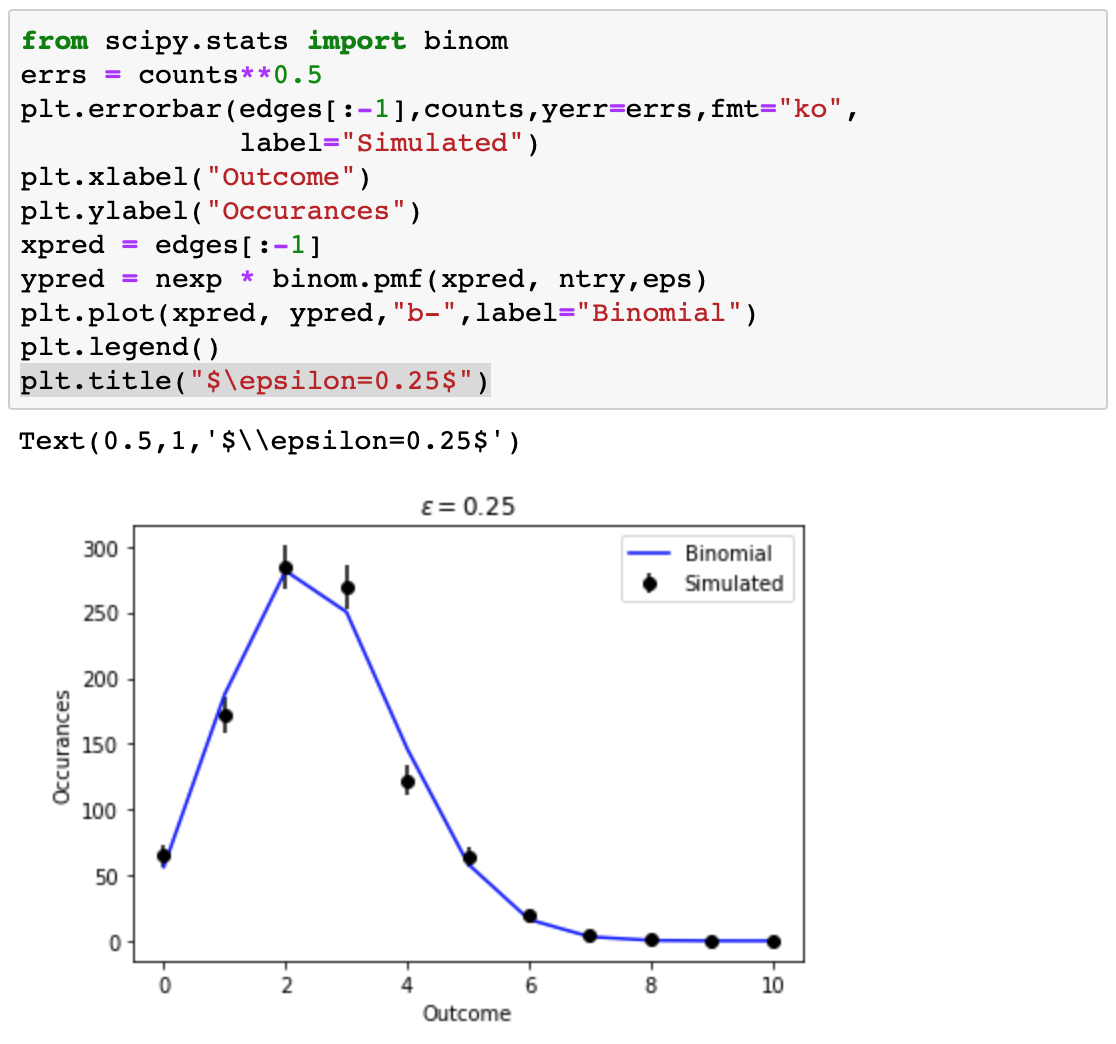
\includegraphics[width=0.85\textwidth]{figs/labs/distributions/compare.png}
\\ Notice that we scale the PDF by the number of experiments $n_{\rm
  exp}$.  The PDF is the expected frequency of each outcome for a
single experiment, but we are plotting the number of occurrences for
$n_{\rm exp}$ experiments.

\begin{plot} Compare the output of your Monte Carlo simulation
with the Binomial distribution PDF with $n_{\rm exp} = 1000$ and
$n_{\rm try} = 10$, and $\epsilon = 0.75$. See example for $\epsilon = 0.25$ in the plot above.
%and for three different values of $\epsilon$:
%0.25, 0.5, and 0.75.  For example, Plot 1 should look like the plot above. 
\end{plot}


\section{The Poisson Limit}

The Poisson distribution follows from the Binomial distribution in the
limit that $n_{\rm try} \to \infty$.  Recall that the mean value of
the Poisson distribution is $\bar{m} = \epsilon \, n_{\rm try}$.  If
we kept the success rate $\epsilon$ as a parameter, than any finite
value of $\epsilon$ would cause the mean of the distribution to diverge to infinity.
If instead we hold the new parameter $\lambda$ constant, and set:
\begin{displaymath}
\epsilon = \frac{\lambda}{n_{\rm try}}
\end{displaymath}
we see that $\epsilon \to 0$ as $n_{\rm try} \to \infty$ and the mean
of the Poisson distribution remains at the fixed value $\lambda$.

We'll explore this limit numerically simply by taking $n_{\rm try}$ to
the large (but finite) value of 1000.  Re-run your Monte Carlo
simulation using the parameters $n_{\rm try} = 1000$, $n_{\rm exp} =
1000$, and $\epsilon = \lambda / n_{\rm try}$.  For now, take $\lambda
= 2.0$.  Instead of the Binomial distribution, compare your simulation to the Poisson distribution PDF
using the {\tt poisson.pmf} function:
\begin{verbatim}
from scipy.stats import poisson
xpred = edges[:-1]
ypred = nexp * poisson.pmf(xpred, lamb) 
\end{verbatim}
Note that the first argument of the {\tt pmf} function is the array of
positions to evaluate the function at, while the second is the Poisson
parameter $\lambda$.  Also note that sadly {\tt lambda} is a reserved word
in python, and so you cannot use it as a variable name.

\begin{figure}[htbp]
\begin{center}
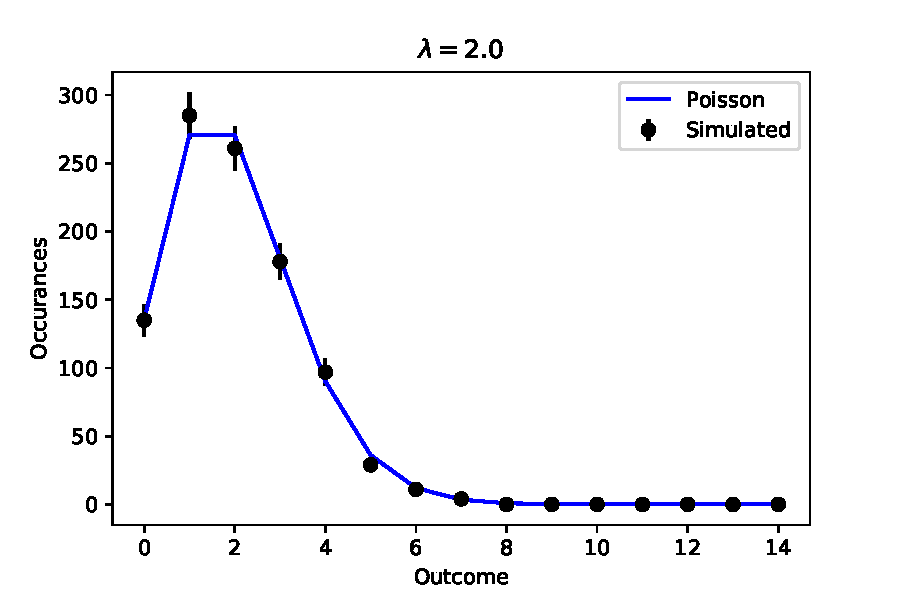
\includegraphics[height=0.22\textheight]{figs/labs/distributions/poisson.pdf}
\end{center}
\caption{\label{fig:poisson} Example of the expected result for the Monte Carlo simulation data in comparison to the Poisson PDF for for $\lambda=2$. }
\end{figure}

\begin{plot} In the Poisson limit, compare the output of your Monte Carlo simulation to the Poisson PDF
for $\lambda=5.2$.
%for two different values of $\lambda$:  2.0, 5.2.  
Plot the histogram with 15 bins for the outcomes: 0,1,2,3,...,14.  
An example for $\lambda=2$ is shown in Fig.~\ref{fig:poisson}.
\end{plot}

%Using {\tt np.mean} and {\tt np.var}, check that mean and variance of
%your distributions is as you expect in each case, and record the
%results in your log book.

This is a \textbf{sign-off point} for this lab.  Make certain you can
explain your code, and that it is as neat and organized as you can
manage.

\section{The Gaussian Limit}

\begin{figure}[htbp]
\begin{center}
\begin{tabular}{cc}
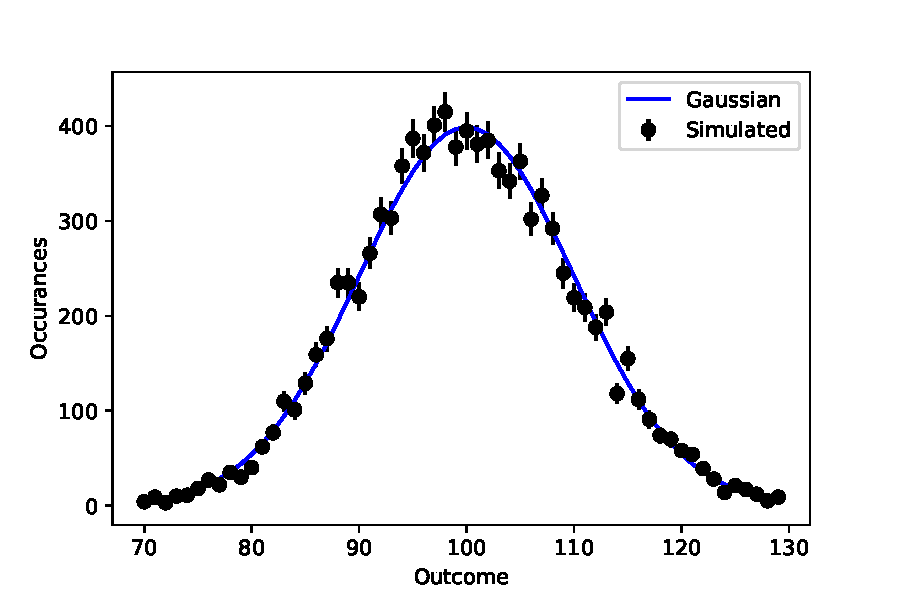
\includegraphics[height=0.22\textheight]{figs/labs/distributions/gauss_finebins.pdf} &
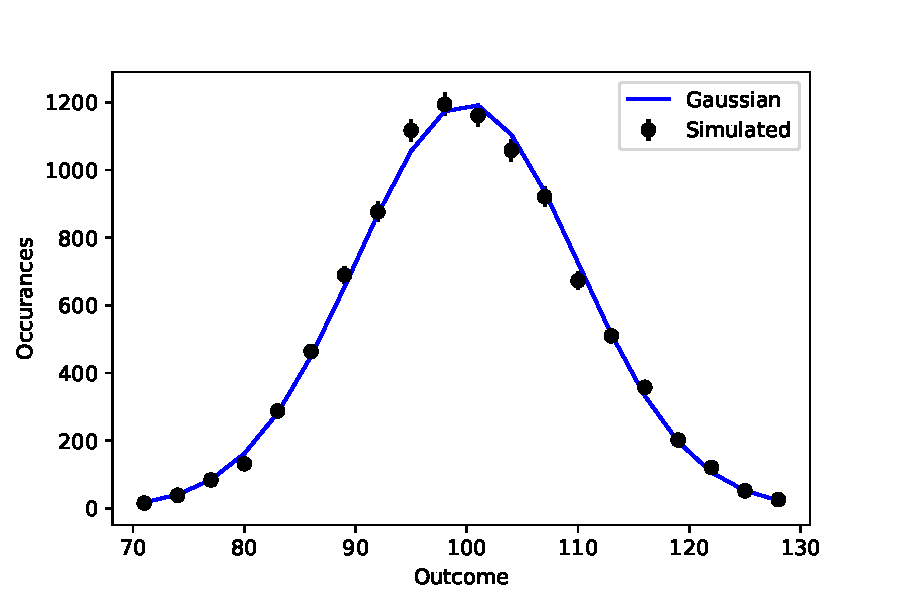
\includegraphics[height=0.22\textheight]{figs/labs/distributions/gauss.pdf} \\
(a) & (b) \\
\end{tabular}
\end{center}
\caption{\label{fig:gauss} Example of the expected result for the Monte Carlo simulation data in comparison to the Gaussian PDF for $\lambda=100$. }
\end{figure}

As the mean value $\lambda$ of the Poisson distribution gets larger,
the Poisson distribution resembles the Gaussian distribution.  We will
simulate this numerically by taking our Monte Carlo simulation in the
Poisson limit, as above, with $\lambda = 100$.  Initially use
integer bins inclusively in the range 70 to 130, e.g.:
\begin{verbatim}
counts,edges = np.histogram(m,bins=60,range=(70,130))
\end{verbatim}
and compare with the Gaussian (also called normal) distribution PDF, e.g.:
{\tt scipy.stats.norm.pdf} function:
\begin{verbatim}
from scipy.stats import norm
xpred = edges[:-1]
ypred = nexp * norm.pdf(xpred, loc=lamb, scale=lamb**0.5). 
\end{verbatim}

\begin{plot} Set the parameter {\tt loc} to the mean value, and the parameter {\tt
  scale} to $\sigma$.  Recall that in the Poisson limit $\sigma^2 =
\lambda$, which is why we set {\tt scale=lamb**0.5} in the example.
This should reproduce the plot in Fig.~\ref{fig:gauss}a. \end{plot}

You should see that 60 bins is rather unwieldy.  We'll reduce the number
of bins, but that's actually a bit more complicated than you might
expect: non-integer bins with discrete data is about the most
challenging binning you can tackle.  You'll have to do the following:
\begin{itemize}
\item While keeping the range of 70 to 130, set the number bins to {\tt bins=20} when filling your histogram.
\item Our trick to use edges[:-1] will no longer work, since now the data for each bin is associated with a range of values in the bin.  Each bin is now 3 integers wide. If we live this as is, edges[:-1] will position the x value of the bin at its leading edge: 70, 73, 76 , ......  and the data will be plotted with an observable bias.  For continuous data, we often simply use the middle of the bin:
\begin{verbatim}
cbins = (edges[:-1] + edges[1:])/2.  
\end{verbatim}
This would position the x value of the bins at 71.5, 74.5. 77.5, ..... and that seems more reasonable choice. 
In this specific case of discrete data which doesn't extend  all the way to the right edge this is still slightly biased. The first bin in our example represents the count of all outcomes in the range from 70 (inclusive) to below 73 (exclusive). So its center should be at 71.  To be precise for this specific case, the x position we should use for plotting the contents of each bin is:
\begin{verbatim}
cbins = (edges[:-1] + edges[1:] -1 )/2 
\end{verbatim}
\item The normalization of the PDF to the data now requires an additional scale factor to account for the wider bins (which integrate more probability).  You need to scale by an additional factor of 3 to account for the fact that each bin is 3 integers wide.
\end{itemize}

\begin{plot} Using the techniques described above, reproduce Fig~\ref{fig:gauss}b, which shows that the Binomial distributions becomes a Gaussian distribution as the mean value of the distribution becomes large. \end{plot}

























\chapter{The Central Limit Theorem and Experimental Uncertainties}

%
% TODO:  Students were confused about how to handle bin position
% for plotting discrete data...  some clarification (text, figures) is needed.
%

\section{Introduction}

In this lab, you will produce a numerical demonstration of the central
limit theorem.  You will also model the propagation of uncertainties
and compare with the calculated uncertainties. For this lab there are only jupyter notebook entries. 


\section{Sampling Distributions}

\begin{figure}[htbp]
\begin{center}
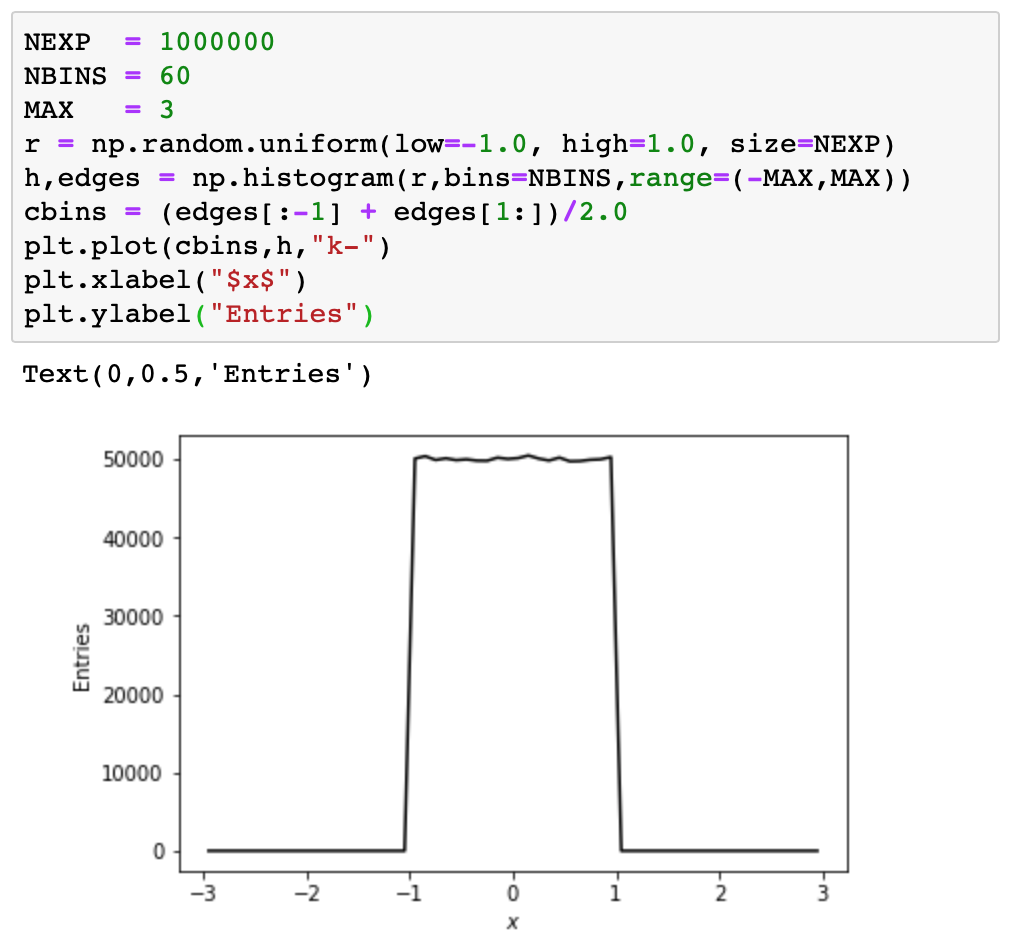
\includegraphics[width=0.75\textwidth]{figs/labs/uncertainties/step.png}\\
\end{center}
\caption{\label{fig:samplingstep} Sampling from the uniform distribution. }
\end{figure}

\begin{figure}[htbp]
\begin{center}
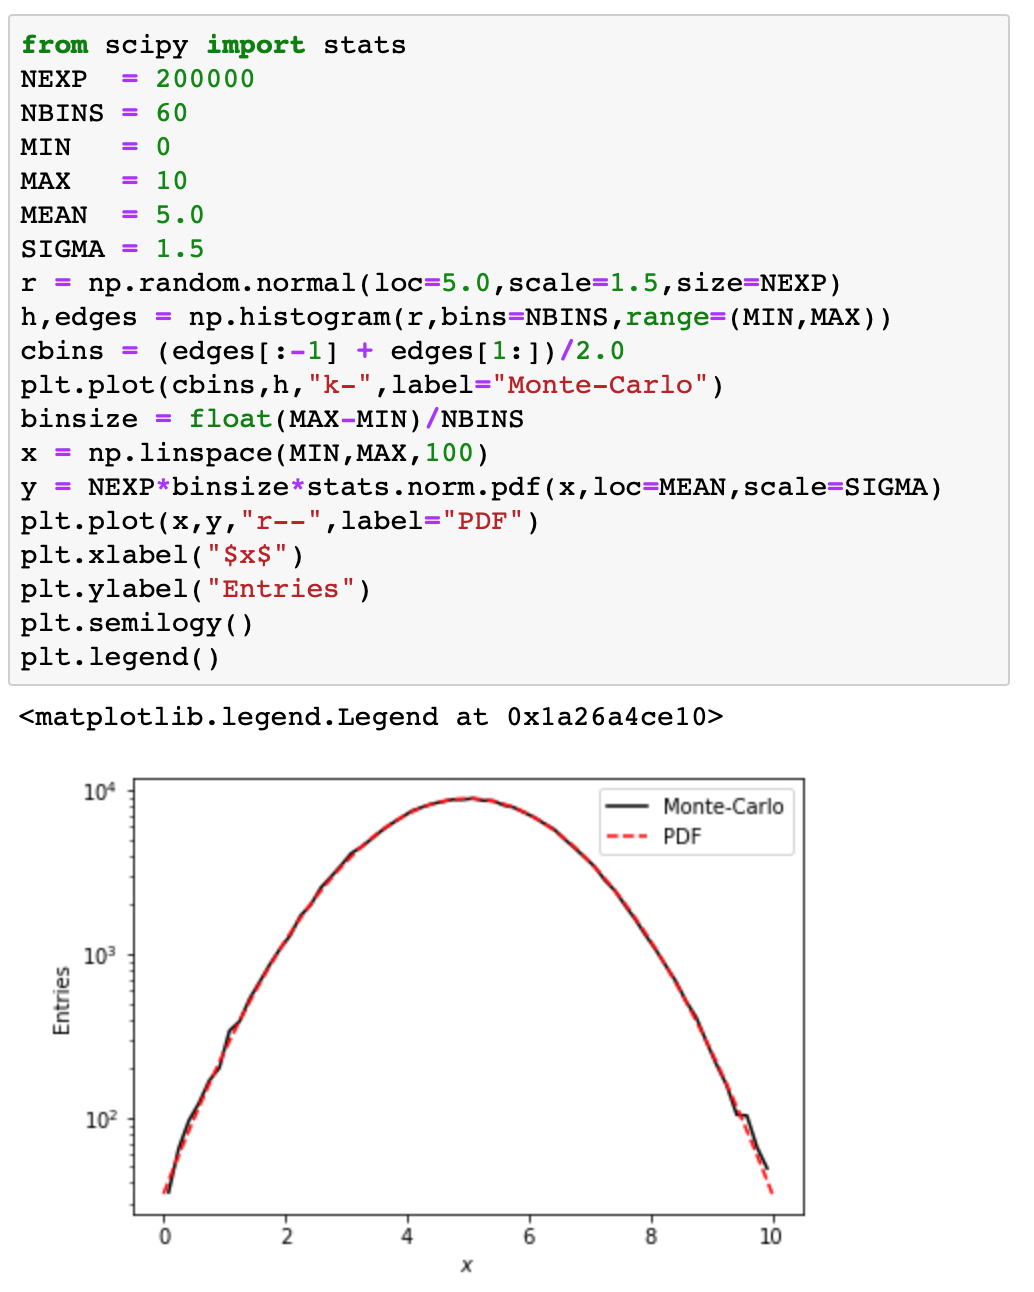
\includegraphics[width=0.75\textwidth]{figs/labs/uncertainties/gaussian.png}\\ 
\end{center}
\caption{\label{fig:samplinggauss} Sampling from the Gaussian distribution and comparison with the Gaussian PDF.}
\end{figure}

Scientific python provides functions to draw random samples according
to various distributions.  In today's lab, we will draw samples
uniformly in the interval $[-1,1]$, as demonstrated in Fig.~\ref{fig:samplingstep}.   The line
\begin{verbatim}
r = np.random.uniform(low=-1.0, high=1.0, size=NEXP)
\end{verbatim}
creates a NumPy array {\tt r} which contains {\tt NEXP} entries, with
each entry chosen uniformly and randomly in the range from -1 to 1.
In the example, these events are displayed in a histogram.  When
plotting histograms with plenty of statistics (one million entries
here) and fine binning (60 bins here) it is usually preferable to use
lines instead of points with error bars for plotting the histograms,
as is done in this example.  Notice, however, that even with one
million events, there are still statistical fluctuations which prevent
the curve from being perfectly smooth.

In Fig.~\ref{fig:samplinggauss}, entries are instead drawn from the Gaussian distribution with the line:
\begin{verbatim}
r = np.random.normal(loc=5.0,scale=1.5,size=NEXP).
\end{verbatim}
The histogram is plotted with a logarithmic $y$ scale:
\begin{verbatim}
plt.semilogy()
\end{verbatim}
which results in the Gaussian distribution appearing as a parabola.  The histogram is compared to the Gaussian PDF appropriately normalized:
\begin{verbatim}
x = np.linspace(MIN,MAX,100)
y = NEXP*binsize*stats.norm.pdf(x,loc=MEAN,scale=SIGMA)
\end{verbatim}


\section{Demonstration of the Central Limit Theorem}

In this section, you'll show that average value of random variables
chosen uniformly from -1 to 1 approaches a Gaussian distribution,
consistent with the central limit theorem.  First create a 2-D array
of size {\tt NEXP} by {\tt NAVG} filled with uniform random values in
the interval from -1 to 1, as follows:
\begin{verbatim}
r = np.random.uniform(low=-1.0, high=1.0, size=(NEXP,NAVG))
\end{verbatim}
Then calculate averages values from {\tt NAVG} entries:
\begin{verbatim}
x = np.sum(r, axis=1)/float(NAVG)  
\end{verbatim}
From the Central Limit Theorem, we expect the entries in x to approach a Gaussian distribution.

\begin{plot}  Set {\tt NEXP} to 1000000 for plenty of statistics.
Produce three different histograms with 40 bins covering the range
from -1.2 to 1.2 for three values {\tt NAVG}: 1,2, and 3.  Plot all
three histogram in the same graph with appropriate legend. \end{plot}

Your plot will show that already for three contributions to the average, the result looks quite Gaussian on a linear scale.  For more precise comparison, will use a log scale and compare to the PDF.

\begin{plot} Calculate {\tt NEXP}$=1000000$ average values {\tt x} for {\tt NAVG}$=10$.  Calculate the mean value of the entries in {\tt x} using the {\tt np.mean} function.  Calculate $\sigma$ for the entries in $x$ by taking the square root of the output from the {\tt np.var} (variance) function.  Produce a histograms with 20 bins covering the range
from -0.5 to 0.5 for the average values.  Compare with a Gaussian distribution, appropriately normalized, using your calculated values from the  mean and sigma.  Plot both the histogram and PDF on the same graph, including an appropriate legend.  Use a logarithmic $y$ axis. \end{plot}


\section{Propagation of Uncertainties}

\begin{figure}[htbp]
\begin{center}
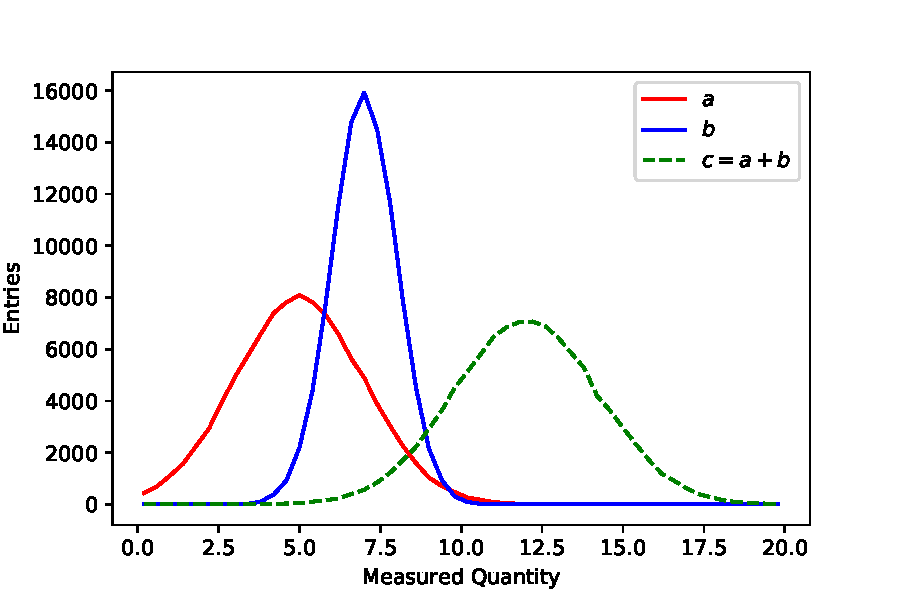
\includegraphics[width=0.75\textwidth]{figs/labs/uncertainties/addunc.pdf}\\
\end{center}
\caption{\label{fig:addunc} Simulation of many measurements of the quantity $c = a + b$. }
\end{figure}

Consider two measured values $a \pm \sigma_a$ and $b \pm \sigma_b$.  If we calculate the quantity $c = a + b$ or $c = a - b$, the uncertainty on the calculated value $c$ is given by:
\begin{displaymath}
\sigma_c = \sqrt{\sigma_a^2 + \sigma_b^2}.
\end{displaymath}
If instead, we calculate $c = a * b$ or $c = a/b$ the fractional uncertainty on $c$ is given by:
\begin{displaymath}
\frac{\sigma_c}{c} = \sqrt{\left(\frac{\sigma_a}{a}\right)^2 + \left(\frac{\sigma_b}{b}\right)^2}.
\end{displaymath}
In this section, you'll develop a numerical simulation for the
propagation of uncertainties under addition, subtraction,
multiplication, and division.  An example, for $c = a + b$ is shown in Fig.~\ref{fig:addunc}.

\begin{print} Pick values for $a$, $b$, $ \sigma_a$ and $ \sigma_b$ for simulating subtraction: $c=a-b$. Print them out in your notebook. Choose the values that are different from what is plotted in Fig.~\ref{fig:addunc}.  \end{print}

\begin{plot} 
Simulate the measurement $a$ by drawing 100,000 random variables
sampled from the Gaussian distribution with mean $a$ and sigma
$\sigma_a$, and likewise for $b$.  Calculate the values of $c = a -b $ from
the $a$ and $b$ values.  Plot the result in histogram with 50 bins and an appropriate range. \end{plot} 

\begin{print} 
Calculate the mean and variance of the mean and variance of the simulated $c$ values and compare to your expectations for the mean, variance of the distribution and variance of the mean. Apply the standard propagation of uncertainties for calculating expectation value for the variances. 
 \end{print}


This is a \textbf{sign-off point} for this lab. 

\begin{print} Pick values for $a$, $b$, $ \sigma_a$ and $ \sigma_b$ for simulating division: $c=a/b$. Print them out in your notebook.  Choose the values that are different from what is plotted in Fig.~\ref{fig:addunc}.  \end{print}

\begin{plot} 
Simulate the measurement $a$ by drawing 100,000 random variables
sampled from the Gaussian distribution with mean $a$ and sigma
$\sigma_a$, and likewise for $b$.  Calculate the values of $c = a/b $ from
the $a$ and $b$ values.  Plot the result in histogram with 50 bins and an appropriate range. \end{plot} 

\begin{print} 
Calculate the mean and variance of the mean and variance of the simulated $c$ values and compare to your expectations for the mean, variance of the distribution and variance of the mean. Apply the standard propagation of uncertainties for calculating expectation value for the variances. 
 \end{print}

 
%{\bf Plot 3-6:}  Produce four plots simulating addition, subtraction, multiplication, and division, as in Fig.~\ref{fig:addunc}.  In each case, compare the measured variance of the $c$ values with your expectation.































\chapter{Curve Fitting}
%ADD CHI2 calculation 
\section{Introduction}

In this lab, you will learn about curve fitting with Scientific Python
function {\tt curve{\_}fit}.  For this lab there are only jupyter notebook entries. 

Given a function to fit $f(x;p)$, with p
representing any number of parameters, and a set of measurements $y_i$ and points $x_i$,
the {\tt curve{\_}fit} function determines the best fit parameters by
minimizing:
\begin{equation}
\chi^2 = \sum_i \frac{(f(x_i;p) - y_i) ^2}{\sigma_i^2}.
\label{eqn:chi2}
\end{equation}
If the uncertainties $\sigma_i$ are not specified, the function
assumes $\sigma_i = 1$, and still finds the correct minimum
if the actual uncertainties are identical to one another.

\section{Fitting a Straight Line}

\begin{figure}[htbp]
\begin{center}
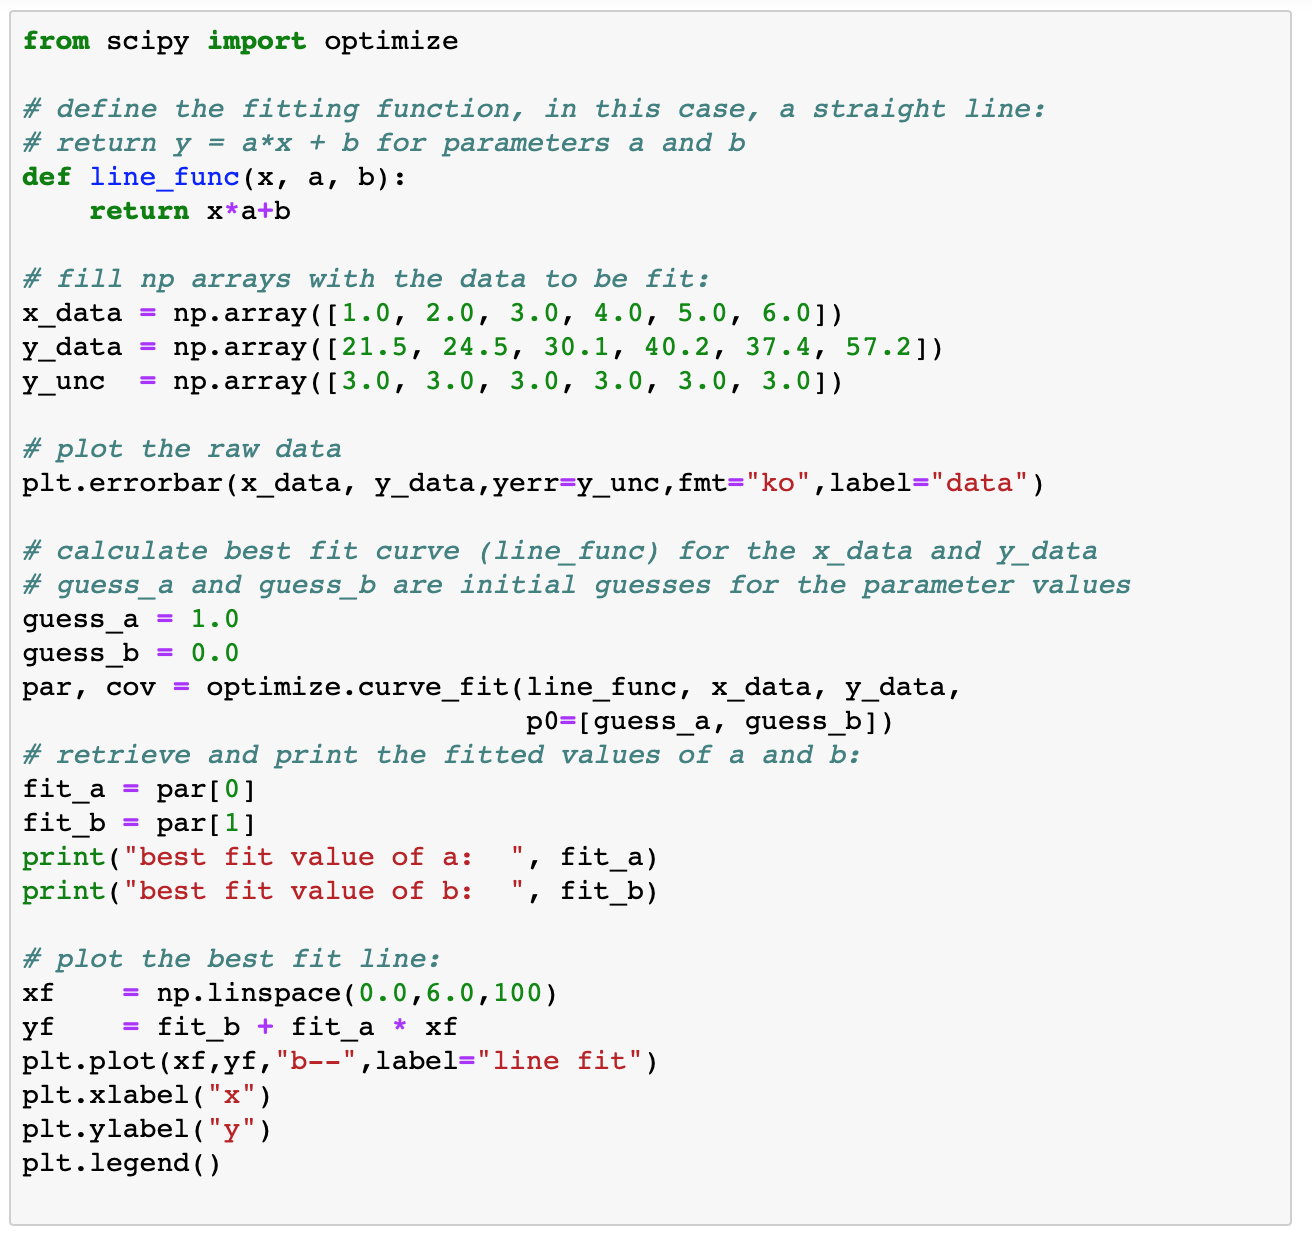
\includegraphics[width=0.65\textwidth]{figs/labs/fitting/fit_code.png} \\
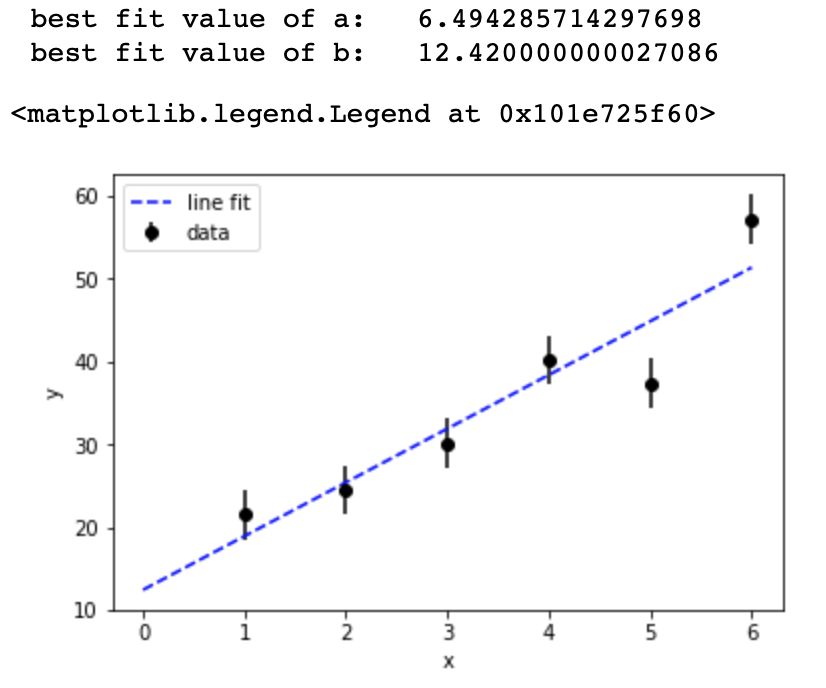
\includegraphics[width=0.65\textwidth]{figs/labs/fitting/fit_out.png} \\
\caption{Example fitting data to straight line.}
\label{fig:fiteg}
\end{center}
\end{figure}

An example using Scientific Pythons {\tt curve{\_}fit} function to fit
a straight line to data is shown in Fig.~\ref{fig:fiteg}.  A block of 
code defining the function we wish to fit, in this case, a straight
line, is defined as a function:
\begin{verbatim}
     def line_func(x, a, b):
         return a*x + b
\end{verbatim}
In this case, the function requires three parameters (in the computer
science sense) the x data in a numpy array as function parameter x,
the slope as function parameter a, and the intercept as function
parameter b.  When called, the function returns the x data multiplied
by the value a, with the value b added.  We don't directly call this
function, but in principle, it could be called like:
\begin{verbatim}
    y_data = line_func(x_data, 2.0, 0.0)
\end{verbatim}
to create a numpy array {\tt y{\_}data} constructed from {\tt
  x{\_}data} with slope 2 and intercept 0.

The next section filling numpy arrays containing the data, and
plotting it with error bars should be familiar by now.  The fit itself
is performed by the line:
\begin{verbatim}
par, cov = optimize.curve_fit(line_func, x_data, y_data, p0=[guess_a, guess_b])
\end{verbatim}
This performs a fit of the function {\tt line{\_}func} defined above
to the $x$ and $y$ data contained in the arrays {\tt x{\_}data} and
{\tt y{\_}data}.  Numerical fits generally find the local minimum,
which is not necessarily the global minimum of interest.  It is
important therefore, especially for complicated fits, to provide an
initial guess near the expected fit values.  These are provided to the
optional, named, function parameter {\tt p0}, which is set to the
python list {\tt [guess{\_}a, guess{\_}b]} which contains our initial guesses for
the fit parameters $a$ and $b$.  The function performs a least-squares
fit to find the best values of $a$ and $b$ which are returned as the
numpy array {\tt par}.  The function also returns the covariance
matrix as the numpy array {\tt cov}.

The remaining code simply uses the best fit values to plot the fitted
function as a dashed line.  Numerical fits are fickle.  Even if you
are only interested in the fitted value, you should always plot the
best-fit function and compare the results to your data as in important
check for your work.

\begin{table}
\caption{Sample data for straight line fit.}
\label{tbl:linesamp}
\begin{center}
\begin{tabular}{ll}
$x$ & $y \pm \sigma_y$ \\
1.0  & $15.9 \pm 3.0$ \\
2.0  & $23.6 \pm 3.0$ \\
3.0  & $33.9 \pm 3.0$ \\
4.0  & $39.7 \pm 3.0$ \\
5.0  & $45.0 \pm 10.0$ \\
6.0  & $32.4 \pm 20.0$ \\
\end{tabular}
\end{center}
\end{table}

%\begin{figure}[htbp]
%\begin{center}
%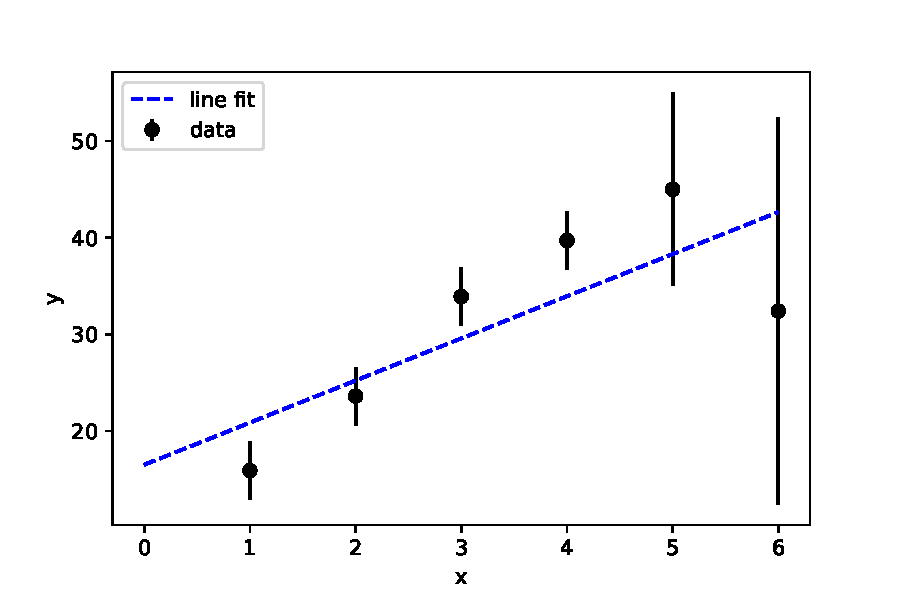
\includegraphics[width=0.65\textwidth]{figs/labs/fitting/bias.pdf} 
%\caption{This linear fit is biased by the failure to properly account for uncertainties.}
%\label{fig:fitbias}
%\end{center}
%\end{figure}

\begin{plot} Apply a code like that of Fig.~\ref{fig:fiteg}
to the data in Table~\ref{tbl:linesamp}. Plot the data including error bars and the best-fit function.
% reproduce the plot in Fig.~\ref{fig:fitbias}.  
\end{plot}

Notice that the last two data points have larger uncertainties than
the other data points.  However, the call to the {curve{\_}fit}
function does not provide the parameter uncertainties, and so the
function assumes that they all have the value $1$.  In this case,
since the uncertainties are not in fact all the same, the function
does not find the correct minimum.  The answer is clearly biased
toward the poorly measured points, because the function gives these
points the same weight as all of the other points.

\begin{print} The {\tt curve{\_}fit} function does not provide directly the $\chi^2$ value of the fit. However you can calculate it manually via equation~\ref{eqn:chi2}. The sum can be obtained via numpy function sum. Modify your code to include calculation of the $\chi^2$ value of the fit. Include also the calculation of the $\chi^2$ divided by the number of degrees of freedom (number of data points minus number of parameters), which is called reduced $\chi^2$. Print both of those values. Is the fit reasonable based on the reduced $\chi^2$ value? Print your comment as well. 
\end{print}

\begin{plot} Look-up the {\tt curve{\_}fit} function and the optional parameter
{\tt sigma}. Provide the correct uncertainties to
the fit and make a new plot with the data and the fit.  You should observe that the fit results is no longer biased,
and more closely tracks the well constrained left side of the plot. \end{plot}

\begin{print} Print $\chi^2$ and reduced $\chi^2$ value. Is the fit reasonable based on the reduced $\chi^2$ value? Print your comment as well. \end{print}

\section{Parameter Uncertainties I}
\label{sec:sigmatrue}
As discussed in the lecture the uncertainty $\sigma_{p_i}$ on the $i$th parameter $p_i$
can be determined from the second derivative of the $\chi^2$ function:
\begin{displaymath}
\frac{d^2\chi^2}{d p_i^2} = \frac{2}{\sigma_{p_i}^2}.
\end{displaymath}
In general, for $M$ parameters, the $M \times M$ covariance matrix is calculated as:
\begin{displaymath}
C(i,j) = 2 \cdot \left(\dfrac{d^2\chi^2}{d p_i d p_j} \right)^{-1}
\end{displaymath}
from which we can see that the diagonals are simply the parameter uncertainties squared:
\begin{displaymath}
C(i,i) = 2 \cdot \left(\dfrac{d^2\chi^2}{d p_i^2} \right)^{-1} = \sigma^2_{p_i}.
\end{displaymath}
The off-diagonal elements contain information about how parameters are
correlated, and for a well designed fit function they should be close to
zero.

The {\tt curve{\_}fit} function returns both the best fit parameter values and the covariance matrix:
\begin{verbatim}
par, cov = optimize.curve_fit(...)
\end{verbatim}
For a fit with $M$ parameters, we can obtain an array containing the
$M$ parameter uncertainties from the square root of the diagonals of the $M \times M$
covariance matrix:
\begin{verbatim}
unc = np.sqrt(np.diag(cov))
\end{verbatim}

We can obtain uncertainties of parameters by accessing elements of the array.

Lets study this in an example for $N=1$ parameter. Generate $x$-values as a numpy array of evenly spaced values from 0 to 99. Generate $y$-values as 100 random numbers drawn from a Gaussian distribution with mean $m = 50$ and a width $\sigma_y =10$.  Perform a fit using {\tt curve{\_}fit} function. Set the uncertainties on the $y$ values to 10 and also set parameter {\tt absolute{\_}sigma = True}.  

 The best fit constant value we expect is simply the mean of the $y$-values.  The
uncertainty on the mean value should be:
\begin{displaymath}
\sigma_m = \sigma_y / \sqrt{N} = 10 / \sqrt{100} = 1.0
\end{displaymath}

\begin{print} Calculate the expected values for the best fit value and its uncertainty. Print them together with the fitted best fit value and its uncertainty. Do those agree? \end{print}


\section{Fitting a Sine Curve}

In this section, you will fit the sample data to a sine function:
\begin{displaymath}
 y = A \, \sin( k x). 
\end{displaymath}
Use the following sample data:\\
\begin{center}
\begin{tabular}{|ll| ll|ll|}
\hline
$x$ & $y$ & $x$ & $y$ & $x$ & $y$\\
\hline
0  & 5.3    & 4  & -9.7   & 8  & 15.7  \\
1  & 15.0   & 5  & -17.4  & 9  & 18.5  \\
2  & 19.2   & 6  & -20.5  & 10 & 8.6   \\
3  & 6.8    & 7  &  2.1   & &  \\
\hline
\end{tabular}
\end{center}
Assume the uncertainty is the same for each $y$ value: $\sigma_i = 2$.
\begin{plot} Plot the data including error bars and the best-fit
sine wave. \end{plot}

\begin{print} Print the best fit parameter
values and their uncertainties. \end{print}

Remember to set {\tt absolute{\_}sigma=True}.\\

This is a \textbf{sign-off point} for this lab. 

\section{Parameter Uncertainties II}

%\begin{figure}[htbp]
%\begin{center}
%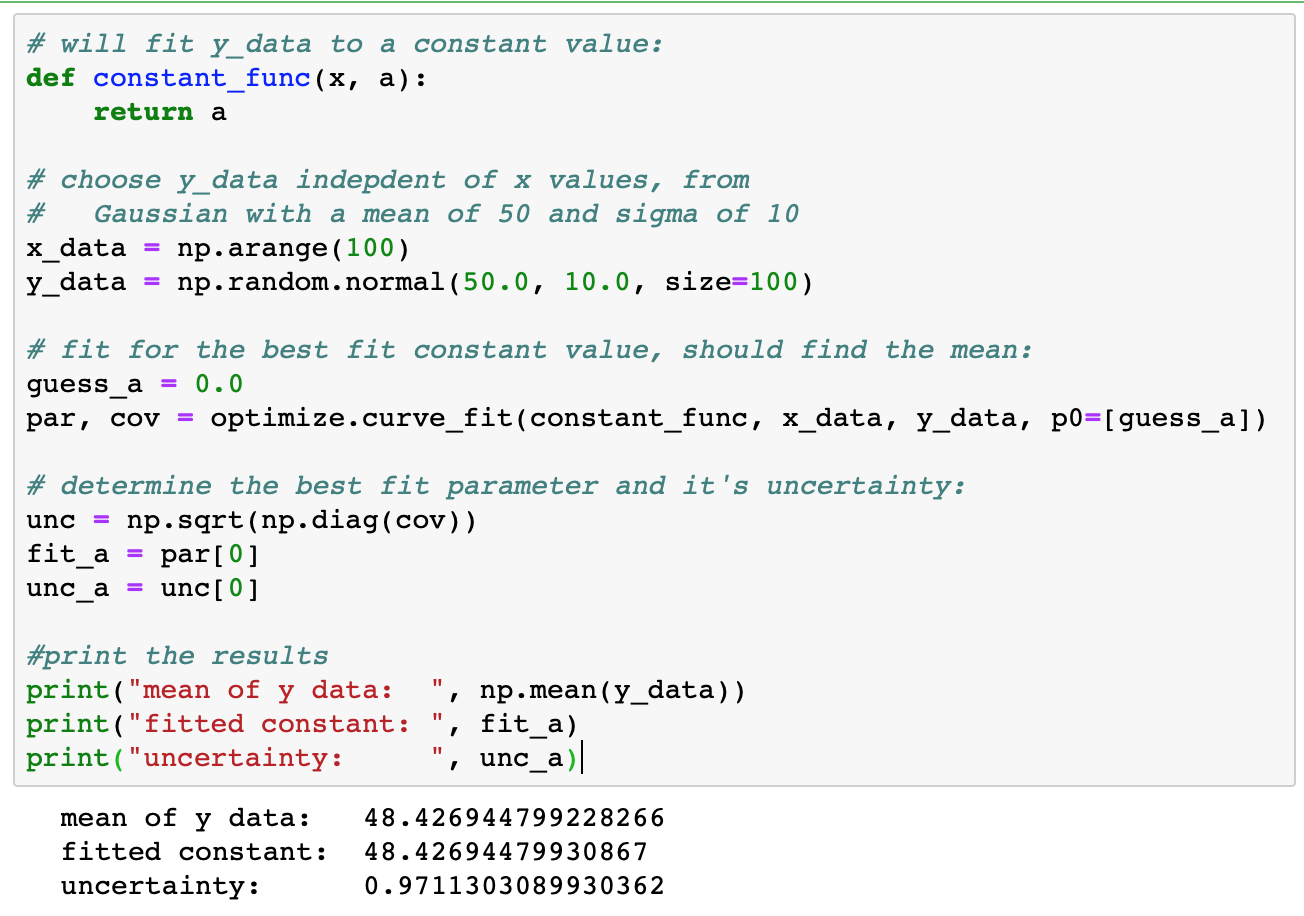
\includegraphics[width=0.65\textwidth]{figs/labs/fitting/uncertainties.png} \\
%\caption{Example obtaining parameter uncertainties.}
%\label{fig:fitunc}
%\end{center}
%\end{figure}

Lets repeat the study in~\ref{sec:sigmatrue}. Generate $x$-values as a numpy array of evenly spaced values from 0 to 99. Generate $y$-values as 100 random numbers drawn from a Gaussian distribution with mean $m = 50$ and a width $\sigma_y =10$.  Perform a fit using {\tt curve{\_}fit} function.  Leave the uncertainties on the $y$ values
unspecified and also leave parameter {\tt absolute{\_}sigma} unspecified. 

\begin{print} Print the fitted best fit value and its uncertainty. \end{print}

It's surprising actually, that the fit returns the correct
uncertainty.  Your code does not provide  the uncertainty on the $y$ parameters $\sigma_y$ to
the fit.  So how can it possible deduce the correct uncertainty
$\sigma_m = \sigma_y / \sqrt{N}$?

The answer is that behind the scenes, the {\tt curve{\_}fit} function
is being really quite clever (too clever, in my opinion, for a default
behavior!)  By default, the covariance matrix returned by the 
{\tt curve{\_}fit} function is scaled by the factor:
\begin{displaymath}
\alpha = \frac{\chi^2_{\rm min}}{\rm NDF}
\end{displaymath}
the minimum value of the $\chi^2$ divided by the number of degrees of
freedom (number of data points minus number of parameters).  As discussed in lecture that $\alpha$ is around 1 for a least-squares fit with
an appropriate model and correct uncertainties.  So nominally this
factor is one, and has no effect.  But consider what happens if the
actual uncertainties are $\sigma$ while the $\chi^2$ used in the fit assumes they
are, for example, ``1''.  In this case, the calculated $\chi^2$ is:
\begin{displaymath}
\chi^2 = \sum_i \frac{(f(x_i;p) - y_i) ^2}{1}
\end{displaymath}
which differs from the correct $\chi^2$:
\begin{displaymath}
\chi^2 = \sum_i \frac{(f(x_i;p) - y_i) ^2}{\sigma^2}
\end{displaymath}
by a factor of $\sigma^2$.  This means that while the correct value
for $\alpha$ is nearly one, the calculated value of alpha will be
$\sigma^2$.  This is precisely the factor needed to scale the squared
parameter uncertainties to account for the fact that the initial
uncertainty was $\sigma$ but we assumed $1$.

This behavior is controlled by the parameter {\tt absolute{\_}sigma}.
By default, the function sets {\tt absolute{\_}sigma = False} and
scales the covariance matrix as just described.  On the other hand, if
you want to simply use the provided uncertainties without re-scaling
the covariance matrix, you must remember to set {\tt
  absolute{\_}sigma = True}.  I think this is a really poor choice of
default behavior...  it's really quite a fancy thing to do implicitly.
In cases when you know the uncertainty on your data points, this
re-scaling actually results in less correct estimate for the
uncertainties.  This is because for a good model with proper
uncertainties, the factor $\alpha$ is near one, but not exactly one.

\begin{print} Repeat the study but leave the uncertainties on the $y$ values
unspecified and set {\tt absolute{\_}sigma = True} in the fit.  You
should obtain an uncertainty of $0.1$.  Print your value and print your explanation of
why you obtained this value. \end{print}

As a rule of thumb, when using {\tt curve{\_}fit}, if you provide
explicit uncertainties, you should remember to set {\tt
  absolute{\_}sigma = True}.  And really, for precision work, you should
almost always be providing explicit uncertainties.



















\end{document}

% OTHER IDEAS:
% Fourier Transforms
% Monte Carlo techniques

